\documentclass[a4paper, 12pt]{book}

\usepackage[T1]{fontenc}
\usepackage[utf8]{inputenc}
\usepackage[italian]{babel}
\usepackage{quoting}
\usepackage{graphicx} %per inserire immagini nel testo
\usepackage{sidecap} %permette di aggiungere didascalie alle immagini
\usepackage{subfig}
\usepackage[colorlinks]{hyperref} %per rendere interattivo il documento, gli elementi interattivi saranno in rosso con l'opzione colorlinks
\usepackage{amsmath}
\usepackage{amsthm} %per enunciati
\usepackage{bohr}
\theoremstyle{plain}
\newtheorem{teorema}{Teorema}[section]
\usepackage{geometry}
\geometry{a4paper, top = 3cm, bottom = 3cm, left = 3.5cm, right = 3.5cm, heightrounded, bindingoffset = 5mm}
\pagestyle{plain}

\author{Giovanni Tosini}
\title{Fisica II}
\date{ }

\begin{document}
\begin{titlepage}
    \maketitle
\end{titlepage}

\frontmatter %numeri romani prima del testo effettivo
\tableofcontents
\mainmatter %numeri arabi dalla prima pagina di testo effettivo

\chapter{Introduzione}

Esistono due tipi di forze in assoluto:
\begin{itemize}
    \item  attrattive
    \item repulsive
\end{itemize}
Queste forze si possono vedere anche nelle singole cariche elettriche, quelle con identica carica
si respingeranno, mentre quelle con carica opposta si attrarranno.

Esistono tre modalità per caricare un oggetto:
\begin{itemize}
    \item strofinio
    \item induzione
    \item contatto
\end{itemize}
Da notare che la carica non dipende dal meccanismo con cui viene creata, ma dai costituenti
della materia.
\begin{center}
    \textbf{\textbf{\bohr{10}{A}
    \setbohr{nucleus-radius=1.5em}}}    
\end{center}
Un atomo è composto da: protoni, neutroni ed elettroni. La differenza di dimensioni tra un protone
e un elettrone è di parecchi ordini di grandezza. La carica elettrica di un elettrone viene 
denominata "carica elementare", è tale perché si dice "quantizzata" essendo che si possono trovare solo
cariche multiple di essa. Inoltre il modulo della carica di un elettrone è equivalente alla carica di
 un protone, sebbene siano due particelle differenti.
 \begin{quote}
     \begin{math}
         |qe^-| = qe^+
     \end{math}
 \end{quote}
 La materia ordinaria è neutra, di conseguenza pure l'atomo è neutro, ovvero il centro di 
 simmetria del nucleo coincide con quello degli elettroni.

 Con lo strofinio vengono strappati gli elettroni meccanicamente, nel sistema isolato d'esempio
 (in un sistema isolato la carica totale Q si conserva) preso in questione. La carica dipenderà 
 dal potenziale di estrazione del materiale.

 Per induzione invece, un oggetto \begin{math}
     q^+
 \end{math} avvicinato a un oggetto neutro, porterà a una divisione di cariche nell'oggetto neutro 
 causato dall'induzione elettrostatica
 \begin{center}
     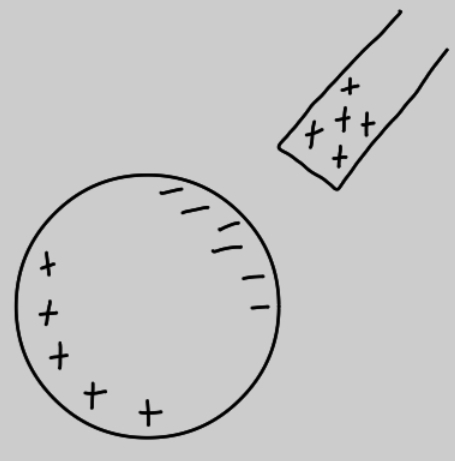
\includegraphics[width=0.5\textwidth]{induzione_elettrostatica.jpg}
 \end{center}

 \chapter{Elettrostatica nel vuoto (in assenza di materia dielettrica)}

Quando non c'è dipendenza dal tempo il campo elettrico e il campo magnetico sono separati.

\section{Interazione (forze) di Coulomb}

\begin{center}
    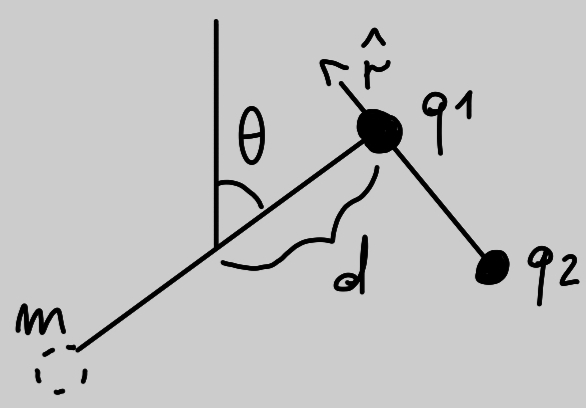
\includegraphics[width=0.5\textwidth]{coulomb.jpg}
\end{center}

\begin{itemize}
    \item m oggetto di massa m, trascurabile
    \item \begin{math}
        \theta
    \end{math} angolo
    \item $q_1$ e $q_2$ sono le cariche
    \item d la distanza
    \item r il versore
\end{itemize}

La forza esercitata lungo d sarà equivalente a:
\begin{quote}
    \begin{math}
        |\vec{F}|=k\frac{q_1q_2}{r^2}
    \end{math}
\end{quote}
Questo è un modello valido \textbf{esclusivamente} per cariche ferme nel vuoto. La costante k 
equivale a
\begin{quote}
    \begin{math}
        k=\frac{1}{4\pi\epsilon_0}
    \end{math}
\end{quote}
Di conseguenza la forza esercitata su $q_1$ sarà equivalente a
\begin{quote}
    \begin{math}
        \vec{F}=\frac{1}{4\pi\epsilon_0}\frac{q_1q_2}{r^{2}_{1,2}}
    \end{math}
\end{quote}

N.B.: \begin{itemize}
    \item l'unità di misura della carica equivale al Coulomb, q = [C].
    \item \begin{math}
        \epsilon_0
    \end{math} è la permeabilità sul vuoto (  costante dielettrica del vuoto)
    \item \begin{math}
        r_{1,2} = \vec{r}_{12} = \vec{r}_2 - \vec{r}_1
    \end{math}
    \item se \begin{math}
        q_1q_2
    \end{math} è positivo allora avremo a che fare con una forza repulsiva, se negativo attrattiva
\end{itemize}

\begin{center}
    \includegraphics*[width=0.5\textwidth]{coulomb_2.png}
\end{center}
\begin{center}
    \includegraphics*[width=0.5\textwidth]{coulomb_3.png}
\end{center}
Una carica $q_0$ in uno spazio vuoto, con attorno N cariche, sarà sotto l'effetto della somma della forza di tutte:
\begin{quote}
    \begin{math}
        \sum_{i = 1}^N \frac{q_iq_0}{4\pi\epsilon_0}\frac{\hat{r}_{i0}}{r_{{i0}^2}}
    \end{math}
\end{quote}
N.B.: \begin{itemize}
    \item l'unità di misura della forza è il Newton [N]
    \item \begin{math}
        \hat{r_{12}} = \hat{r_2 - r_1}
    \end{math}
\end{itemize}

\section{Campo elettrostatico}
\begin{quote}
    \begin{math}
        \vec{F_{q_0}} = q_0\vec{E}_i(\vec{r}_0)
    \end{math}
\end{quote}
dove
\begin{itemize}
    \item $\vec{E}$ è la sommatoria senza $q_0$
    \item $\vec{r}_0$ equivale a $\frac{1}{4\pi\epsilon_0}\frac{q_i}{r^2_{i0}}\hat{r}_i0$
    \item che a sua volta equivale a $\frac{\vec{F}_{q_iq_0}}{q_o}$
    \item $\vec{F}_{q_iq_0} = q_0\vec{E_i}$
    \item $\vec{F}_{tot} = q_0\sum \vec{E}_i$
\end{itemize}

Ogni carica genera un campo.
\begin{quote}
    \begin{math}
        \vec{E}(\vec{r}) = \frac{q}{4\pi\epsilon_0r^2}\hat{r}
        \newline\vec{E}_{tot}(r) = \sum\vec{E}_i = \sum \frac{q_i\hat{r}_{i0}}{4\pi\epsilon_0(r_i-r)^2}
        \newline\vec{F} = q\vec{E}
    \end{math}
\end{quote}
Definizione "operativa" di campo elettrico:
\begin{quote}
    \begin{math}
        \vec{E} = \frac{\vec{F}}{q} [\frac{N}{C}] = [\frac{V}{m}]
    \end{math}
\end{quote}

\section{Energia elettrostatica}

La forza elettrostatica è conservativa? Lo è se:
\begin{itemize}
    \item L non dipende dal percorso
    \item L in un percorso chiuso è nullo
    \item Esiste una funzione di energia potenziale U t.c. L da A->B è uguale a -$\Delta$U
\end{itemize}
\begin{center}
    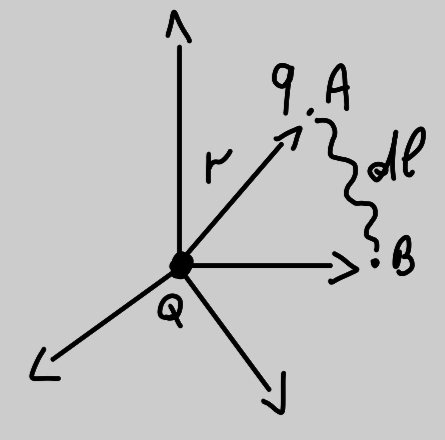
\includegraphics[width=0.5\textwidth]{energia_elettrostatica_1.jpg}
\end{center}
\begin{itemize}
    \item Q è la particella che genera il campo elettrico
    \item q invece è la particella che si sposta da A a B
    \item $dL = \vec{F}\vec{dl}$
    \item $dL = \frac{qQ}{4\pi\epsilon_0r^2}\hat{r}\vec{dl}$
\end{itemize}
$\hat{r}\vec{dl}$ non è nient'altro che la proiezione di $r$ su $dl$ ovvero $dr$
\newline Il lavoro da A a B invece equivale all'integrale
\begin{quote}
    \begin{math}
        L_{AB} = \int^B_A dL = \frac{qQ}{4\pi\epsilon_0} \int^B_A \frac{\hat{r}\vec{dl}}{r^2} = \int^{r_B}_{r_A} \frac{dr}{r^2} 4
        = -\frac{1}{r}|^{r_B}_{r_A}
    \end{math}
    che è uguale a 
    \begin{math}
        \frac{qQ}{4\pi\epsilon_0}(\frac{1}{r_A}-\frac{1}{r_B}) = -\Delta U\\
        \newline U_{carica q} = \frac{qQ}{4\pi\epsilon_0r}+c
    \end{math}
\end{quote}
L'unità di misura dell'energia potenziale è il Joule [J]
\newline $U_\infty = 0$ perché non ci sono cariche
\newline $U = \frac{qQ}{4\pi\epsilon_0r} = -(U_\infty-U_r) = -\Delta U$

\section{Campo potenziale elettrostatico}

\begin{description}
    \item[N.B.:] le cariche sono statiche
    \item[Definizione:] $\Delta_{AB}V=\frac{\Delta U_{AB}}{q}$ 
\end{description}

Il lavoro del campo, lavoro del potenziale:
\begin{center}
    \item $L=-q\Delta V$
\end{center}

L'unità di misura del potenziale è il Volt [V].
Quindi

\begin{center}

    $\Delta U_{energia} = -\int_A^B \vec{F}\vec{dl} \Rightarrow 
\Delta V=V_B-V_A=-\int_A^B\vec{E}\vec{dl}$

\end{center}
Formula per il calcolo del potenziale:
\[
\begin{cases}
V(r_0) = V_0 = 0 & \mbox{solo in alcuni casi} \\
V(r) = -\int_{r_0}^{r} \vec{E} \vec{dl} \\
\end{cases}
\]

Che cammino scelgo per calcolare $E$? Quello più comodo. Ogni carica genera potenziale e un proprio campo.

\begin{center}
	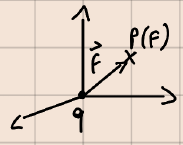
\includegraphics[width=0.5\textwidth]{gr_part.png}
\end{center}      

\[
\begin{split}
	\vec{E} (r) &= \frac{q}{4\pi \epsilon_0 r^2} \hat{r} \\
	&V(r) - V_0 = -\int_{r_0}^{r} \underbrace{\frac{q}{4\pi \epsilon_0 r^2} }_{\vec{E}(r)} \overbrace{\hat{r} \vec{dl}}^{dr} \\
	&-\frac{q}{4\pi \epsilon_0} \int_{r_0}^{r} \overbrace{\frac{1}{r^2}dr}^{=-\frac{1}{r}} \\
	&\frac{q}{4\pi \epsilon_0}[\frac{1}{r} - \frac{1}{r_0}] \\
\end{split}  
\]      

Posso porre $V_0 = 0$ con 

\[
\begin{split}
r_0 &= \infty \\
&V(r) - \underbrace{V_{\infty}}_0 = -\int{\infty}{r} \frac{q}{4\pi \epsilon_0 r^2} = \frac{q}{\pi \epsilon_0 r} \\
&V(r)_q = \underbrace{\frac{q}{4\pi \epsilon_0 r}}_{formula effettiva} [v] con V_{\infty} = 0 \\
\end{split}
\]

$V_{\infty} = 0$ è possibile solo se a $\infty$ non ci sono cariche, ciò è possibile solamente in un sistema finito.  

\paragraph{Cosa succede con N cariche discrete?}

\begin{center}
	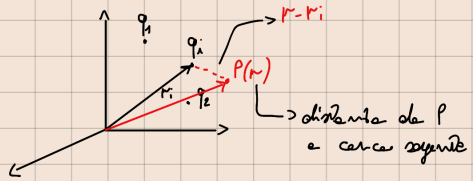
\includegraphics[width=0.5\textwidth]{discrete.png}
\end{center} 

\[
\begin{split}
\vec{E_i}(r) &= \frac{q_i}{4\pi \epsilon_0(r - r_i)^2} \hat{r - r_i} \\
&E_{TOT} = \sum E_i \\
\end{split}
\]

Per il principio di sovrapposizione si possono sommare i campi.

\[
V_{TOT}(r) = \sum_i \frac{q_i}{4\pi \epsilon_0 |r - r_i|}
\]

In una distribuzione continua \[\sum \rightarrow \int\] quindi:
\begin{center}
	\[V(r) = \frac{1}{4\pi \epsilon_0} \int\frac{dq}{r-r'}\]
\end{center}

Che può essere calcolato sullo spazio, il volume o linearmente.

\section{Linee di campo}

Sono linee tangenti al campo in ogni punto, continue ed escono dalle cariche positive mentre entrano da quelle negative.

\begin{center}
	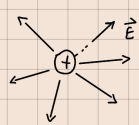
\includegraphics[width=0.5\textwidth]{left.png}
	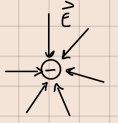
\includegraphics[width=0.5\textwidth]{right.png}
\end{center}

\section{Superfici equipotenziali(superfici in cui V è costante)}
	
\begin{center}
	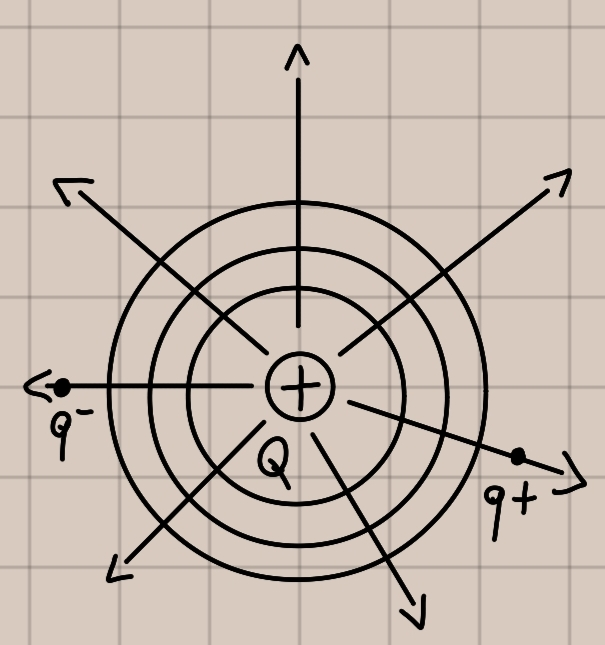
\includegraphics[width=1\textwidth]{equi.jpg}
\end{center}

La carica che genere il campo è circondata da sfere equipotenziali, la carica positiva si sposterebbe fino a \[\infty\] mentre la carica negativa verrebbe attratta fino a scontrarsi con quella che genera il campo.

\[\vec{E}(r) = \frac{\vec{F}}{q} = \frac{Q}{4\pi \epsilon_0 r^2}\hat{r}\]

Si calcoli il lavoro

\[dL = -qdV\] se \[dV = 0\] allora \[dL\] è nullo, implica che la forza generata è perpendicolare alla superficie equipotenziale.

\begin{description}
	\item[N.B.:] il lavoro è negativo quando ci si sposta nella direzione opposta alla forza
\end{description}

Una particella lasciata libera e non fissa nello spazio avrebbe sempre lavoro positivo perché seguirebbe la forza a cui è sottoposta senza farne resistenza.

\begin{description}
	\item[Campo elettrostatico] è conservativo, ovvero esiste una \[V\] t.c. il \[L_q = -\Delta V\]
\end{description}

Il lavoro svolto in un percorso chiuso sarà sempre equivalente a zero, la \textbf{Prima equazione di Maxwell} afferma che:
\begin{itemize}
	\item \[\oint_{\gamma} \vec{E}\vec{dl} = 0 \]
\end{itemize}

\paragraph{Teorema di Gauss}

Viene usato per calcolare \[\vec{E}(r)\] Prendiamo una carica puntiforme $q$. Il campo è costante mantenendo fissa una certa distanza, di conseguenza moltiplicando \[\vec{E}\textrm{ per la superficie della sfera}\] si otterrà una costante.

\begin{description}
	\item[N.B.:] un angolo solido è \[d\Omega = \frac{dS_{sferica}}{r^2} = \frac{\hat{r}\hat{n}dS}{r^2}\]
\end{description}

\paragraph{Flusso del campo $\vec{E}$}

\begin{center}
	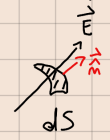
\includegraphics[width=0.5\textwidth]{flusso.png}
\end{center}
\begin{description}
	\item[Flusso elementare] $d\Phi = \vec{E}\vec{dS}$
\end{description}
Dove $\vec{dS} = dS\hat{n}$, il flusso attraverso una superficie equivale a \[\Phi(E) = \int_{sup} \vec{E}\overbrace{\hat{n}dS}^{\vec{dS}}\] che ha come unità di misura \[[\Phi] = [E][superficie] = \frac{V}{m}m^2 = Vm\]
Avremo inoltre che il flusso sarà:
\begin{itemize}
	\item $> 0$ quando il flusso sarà orientato con la normale di $\hat{n}$
	\item $= 0$ quando il flusso sarà perpendicolare alla normale
	\item $< 0$ quando il flusso sarà opposto alla direzione della normale
\end{itemize}

La \textbf{Seconda equazione di Maxwell} afferma che: \[\Phi(\vec{E}) = \oint_{\gamma}\vec{E}\vec{dS} = \frac{Q_{TOT}}{\epsilon_0}\]
Prendendo in considerazione una carica $q$ all'interno di una superficie e concentrandoci solo su una parte della superficie, il flusso generato dalla carica sarà 
\[
\begin{split}
	d\Phi &= \vec{E}\vec{dS}= \\
	&\frac{q}{4\pi\epsilon_0r^2}\hat{r}\hat{n}dS \\
	&\text{notare che}
	\frac{q}{4\pi \epsilon_0}\overbrace{\frac{\hat{r}\hat{n}dS}{r^2}}^{d\Omega} \\
	&\text{di conseguenza} 
	\frac{q}{4\pi \epsilon_0}d\Omega \\
\end{split}
\]
Quindi
\[
\begin{split}
\Phi &= \oint_{\gamma} d\Phi = \\
&\frac{q}{4\pi \epsilon_0}\int_{\gamma}d\Omega = \frac{q}{\epsilon_0}
\end{split}
\]
Aggiungendo altre cariche, il flusso di tutte sarà la somma dei flussi.
\paragraph{Perché le cariche esterne non influenzano?}
Perché il loro flusso è nullo essendo che entrano ed escono dalla superficie.

\section{Elettrostatica nei conduttori}
La sorgente del campo $E$ è una carica ${Q}$, il campo generato 
agisce sulle cariche e queste lo percepiscono, a loro volta ogni 
carica genererà un campo che verrà percepito dalle altre cariche.

La materia neutra affetta da un campo reagirà in due possibili modi:
\begin{itemize}
    \item le cariche libere si metteranno in moto;
    \item i materiali dielettrici vincoleranno le cariche.
\end{itemize}

\subsection{Proprietà di un conduttore in equilibrio}
\begin{SCfigure}[50][h!]
    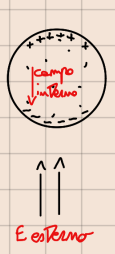
\includegraphics[width=0.3\textwidth]{conduttore.png}
    \caption{Conduttore in equilibrio}
\end{SCfigure}

La  cariche di un conduttore affetto da un campo esterno si 
sposteranno in base alla forza generata dal campo. Con questa separazione
di cariche si accende un campo interno al conduttore, indotto appunto da quello esterno.
Le cariche si sposteranno a fino a quando il campo interno non sarà nullo.

\begin{enumerate}
    \item Il campo interno di un conduttore in equilibrio è $0$, in caso contrario le particelle sarebbero ancora in movimento\[{E_{interno}} = {E_{indotto}} + {E_{esterno}} = 0\];
    \item Il potenziale nel volume del conduttore sarà costante a quello della superficie \[V = \textrm{costante}\]
    \item Se il campo fosse nulle per il teorema di Gauss la carica interna in un conduttore è $0$ \[Q_{interna} = 0\]ha solo carica superficiale \[Q_{superficiale} = \int_{superficie} \sigma dS\]
    \item Il campo della superficie dei conduttori è noto \[\vec{E}_{superficie} = \frac{\sigma}{\epsilon_0}\hat{n}\] è un campo normale alla sua superficie.
\end{enumerate}

\end{document}